\subsection{トルクと粒子の回転}
\label{sec:rotation}
$xy$平面上を$x$軸方向に流れるせん断流下に球形粒子が存在する場合,
流体から受けるトルクは式\eqref{eq:hydro_torque}で表される\cite{hidro_torque}.

    \begin{equation}
        N^\mathrm{H}_z = 4 \pi \mu a^3 \dot{\gamma}
        \label{eq:hydro_torque}
    \end{equation}

\noindent
ここで,$\mu$は流体の粘度,
$a$は粒子の半径,
$\dot{\gamma}$はせん断速度である.
流体から受けるトルクに加えて,
\ref{sec:equation_of_motion}で述べたbottom heavy性によるトルクを考えることで,
粒子の回転の有無を考えることができる.
本研究では,$xy$平面上を$x$軸方向に流れるせん断流を考えたため,
squirmerは$xy$平面上を移動すると考えた.
したがって,squirmerの方向ベクトルは$\theta$を用いて
$\boldsymbol{\hat{e}} = (\sin{\theta}, \cos{\theta}, 0)$
のように表すことができる.
また,系にかかる重力を$y$軸方向下向きとし,
$\boldsymbol{g} = (0, -g, 0)$と表すと,式\eqref{eq:bottom_heavy_torque}は,
式\eqref{eq:bottom_heavy_torque_elements}のように表される.

    \begin{align}
        \boldsymbol{N}^\mathrm{b.h.} &= \frac{4}{3} \pi \rho h \cdot (\sin{\theta}, \cos{\theta}, 0) \times (0, -g, 0) \notag \\
        \therefore N^\mathrm{b.h.}_z &= - \frac{4}{3} \pi \rho h g \sin{\theta}
        \label{eq:bottom_heavy_torque_elements}
    \end{align}

\noindent
これにより,流体から受けるトルクと,bottom heavy性によるトルクの和の$z$成分は,式\eqref{eq:sum_of_torque_z}と表される.

    \begin{align}
        N_z &= N^\mathrm{H}_z + N^\mathrm{b.h.}_z \notag \\
            &= 4 \pi \mu a^3 \dot{\gamma} - \frac{4}{3} \pi \rho h g \sin{\theta}
        \label{eq:sum_of_torque_z}
    \end{align}

\noindent
したがって,粒子の進行方向と粒子にはたらくトルクの$z$成分の関係は,
せん断速度の大きさにより,Fig.\ref{fig:sum_torque}(a)〜(c)のように3種類のグラフで表すことができる.
せん断速度が小さい場合には,bottom heavy性によるトルクが支配的となり,Fig.\ref{fig:sum_torque}(a)のように,
トルクの和が0となる$0 \leq \theta < \pi / 2$の間の角度で粒子の進行方向が固定され,粒子は回転しないことが予想される.
また,Fig.\ref{fig:sum_torque}(b)のように,
流体から受けるトルクの値が,bottom heavy性によるトルクの大きさの最大値となる場合は,
粒子の進行方向は$\theta = \pi / 2$に固定され,粒子は回転しないことが予想される.
せん断速度がその値よりも大きくなると,Fig.\ref{fig:sum_torque}(c)のように,
流体から受けるトルクが支配的となり,粒子が定常的に回転することが予想される.
このように,流体から受けるトルクとbottom heavy性によるトルクの釣り合いから,粒子の進行方向が異方的になることが予想される.

\begin{figure}[H]
    \centering
    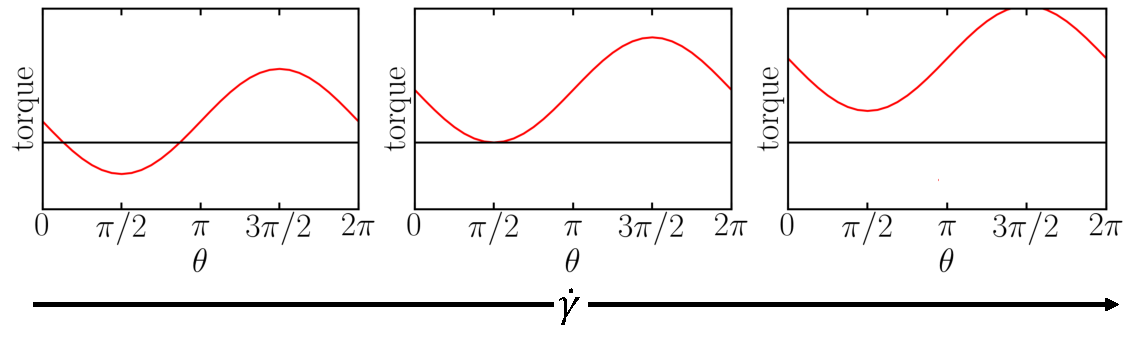
\includegraphics[scale=0.85]{/Users/taiga/Projects/lab/thesis/components/chapter3/figs/sum_torque.pdf}
    \caption{せん断速度の大きさの違いによる粒子にはたらくトルクの分類.
    $\dot{\gamma}_c$は流体から受けるトルクとbottom heavy性によるトルクの絶対値の最大値が等しくなる場合のせん断速度を表す.}
    \label{fig:sum_torque}
\end{figure}
